\nsecbegin{Was wird wie gemacht?}
\nsecbegin{Eclipse}
\nsecbegin{Projekt in Eclipse importieren}
In den workspace wecheln:\\
cd ~/workspace\\
Projekt Klonen:\\
git clone https://gitlab.imn.htwk-leipzig.de/weicker/puml.git\\
Benutzername und Passwort eingeben.\\
In Eclipse "File->Import->Existing Projects into Workspace"\\
%\begin{figure}[hbtp]
%\centering
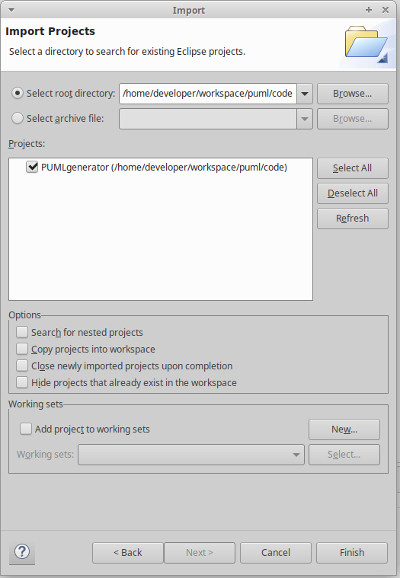
\includegraphics[scale=0.25]{Bilder/importProject}\\
%\caption{Projekt in Eclipse importieren}
%\end{figure}
Dann auf "'Finish"' klicken.
\nsecend

\nsecbegin{WindowBuilder installieren}
In Eclipse "Help->Install New Software..."\\
Unter work with "'2018-09 - http://download.eclipse.org/releases/2018-09"' auswählen.\\
In der Section "'General Purpose Tools"' die im Bild stehenden Häckchen anklicken\\	
\begin{figure}[hbtp]
\centering
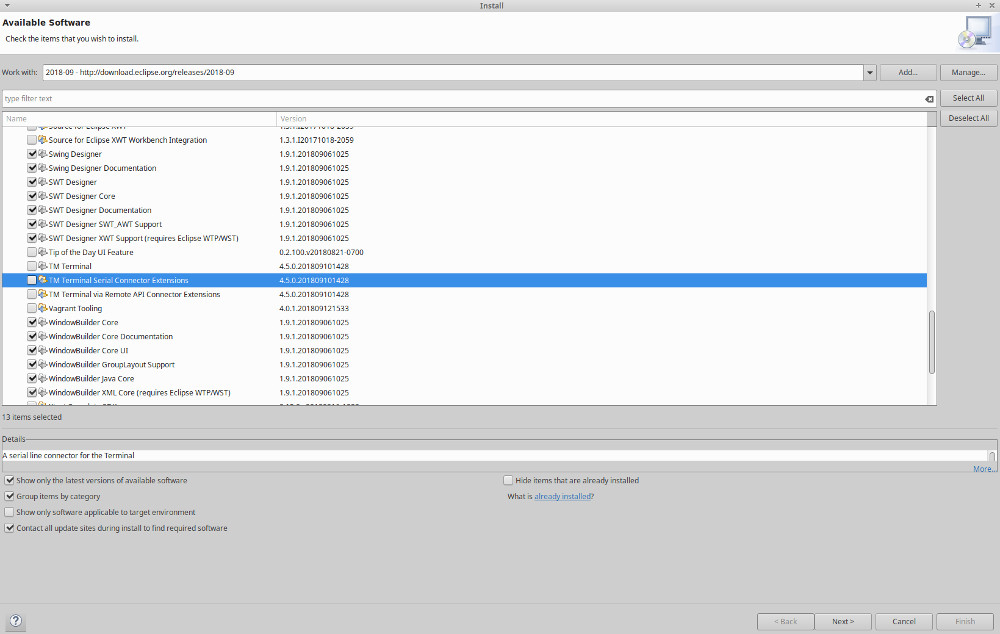
\includegraphics[scale=0.4]{Bilder/installWindowBuilder}\\
\caption{WindowBuilder installieren}
\end{figure}
Dann auf "'Finish"' und sich durch die Installation klicken.
\nsecend

\nsecbegin{GUI editieren}
Es muss der WindowBuilder installiert sein. Dann auf die Datei die die Grafische Oberfläche implementiert (GUI.java) mit der rechten Maustaste klicken. Dann "'Open With->WindowBuilder Editor"' auswählen.
\nsecend
\nsecend

\nsecbegin{LaTeX}
\nsecbegin{Geschachtelte Überschriften}
Durch die Makros:
\begin{itemize}
\item \textbackslash nsecbegin\{MeineÜberschrift\}
\item \textbackslash nsecend
\end{itemize}
können geschachtelte Überschriften verwendet werden. Die Kapitel einfach in diese Makros einschließen. Somit muss nicht darauf geachtet werden auf welcher Ebene man sich im Moment befindet. Dies vereinfacht insbesondere das Auslagern von Text in andere Dateien.\\
Um die Makros in die Autovervollständigung des Texmakers aufzunehmen "'Benutzer/in->Wortvervollständigung anpassen"' wählen und dort die Makros hinzufügen.
\begin{figure}[hbtp]
\centering
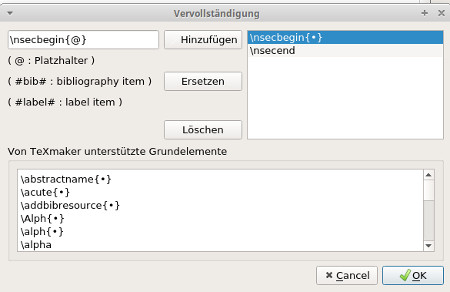
\includegraphics[scale=0.4]{Bilder/autocompleteMakro}
\caption{Autovervollständigung anpassen}
\end{figure}
\nsecend

\nsecbegin{Build-Dateien aufräumen}
Beim erstellen des LaTeX-Dokuments werden jede Menge zusätzliche Dateien erstellt. Dank der entsprechenden "'.gitignore-Datei"' werden diese nicht in GIT hinzugefügt. Für den Fall dass man das Verzeichniss bei sich selbst bereinigen möchte, kann das "'clean.sh"'-Script ausgeführt werden.
\nsecend

\nsecbegin{Entwicklerdokumentation und Handbuch erstellen}
Wenn etwas an der Entwicklerdokumentation oder am Handbuch geändert wurde, müssen diese Dokumente neu erstellt werden. Hierfür zunächst wie gewohnt die LaTeX-Projektdokumentation erstellen. Anschließend kann das "'buildAllDocuments.sh"'-Script ausgeführt werden. Dieses erstellt dann die entsprechenden Dokumente.\\
Weitere Informationen zum "'multiaudience-Paket"' unter \url{https://www.uweziegenhagen.de/?p=3252}.
\nsecend
\nsecend

\nsecend